\begin{figure}[!htb]
  \centering
  \begin{subfigure}[b]{0.1\textwidth}
    \centering
    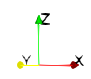
\includegraphics[width=\textwidth]{Chapter5/figures/spallation/orientation_axis}
    \vspace{2em}
  \end{subfigure}
  \begin{subfigure}[b]{0.16\textwidth}
    \centering
    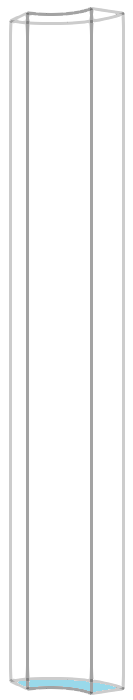
\includegraphics[width=0.6\textwidth]{Chapter5/figures/spallation/geometry_bottom}
    \caption{Bottom}
  \end{subfigure}
  \begin{subfigure}[b]{0.16\textwidth}
    \centering
    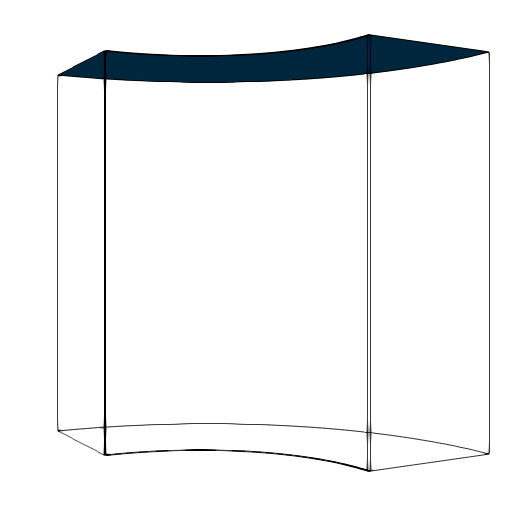
\includegraphics[width=0.6\textwidth]{Chapter5/figures/spallation/geometry_top}
    \caption{Top}
  \end{subfigure}
  \begin{subfigure}[b]{0.16\textwidth}
    \centering
    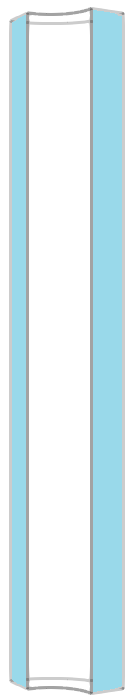
\includegraphics[width=0.6\textwidth]{Chapter5/figures/spallation/geometry_sides}
    \caption{Sides}
  \end{subfigure}
  \begin{subfigure}[b]{0.16\textwidth}
    \centering
    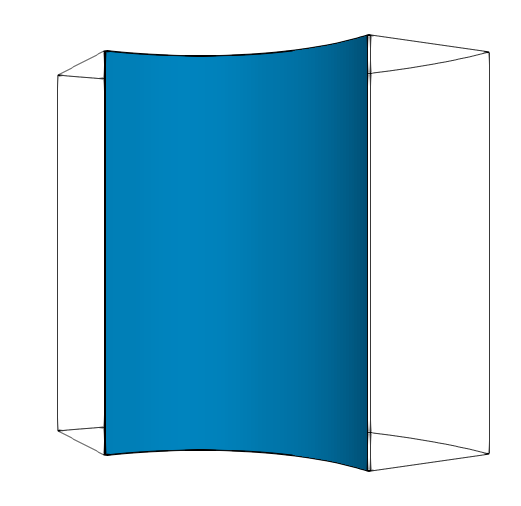
\includegraphics[width=0.6\textwidth]{Chapter5/figures/spallation/geometry_inner}
    \caption{Inner}
  \end{subfigure}
  \begin{subfigure}[b]{0.16\textwidth}
    \centering
    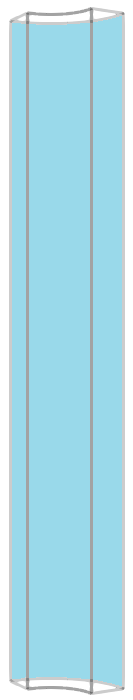
\includegraphics[width=0.6\textwidth]{Chapter5/figures/spallation/geometry_outer}
    \caption{Outer}
  \end{subfigure}
  \caption{Boundaries of the heat exchanger.}
  \label{fig: Chapter5/spallation/boundaries}
\end{figure}
